\namedsection{Initial Design}{Gupta}

The hardware side of this project requires the ARM Cortex M0 processor to obtain the sensor data to classify with the model. The classification then needs to be made visible so a user can see whether they are doing exercise or not, this can be done simply with something such as an LED. During development, it is also useful for debug information to be extracted so it is possible to diagnose issues that may arise as well as test various parts of the system ensuring that they work as expected. 

Figure~\ref{fig:hardware_schematic_development} shows the block diagram for the hardware part of the project whilst still developing and Figure~\ref{fig:hardware_schematic_final} shows the block diagram for the target final system.

\begin{figure}[!hb]
	\centering
	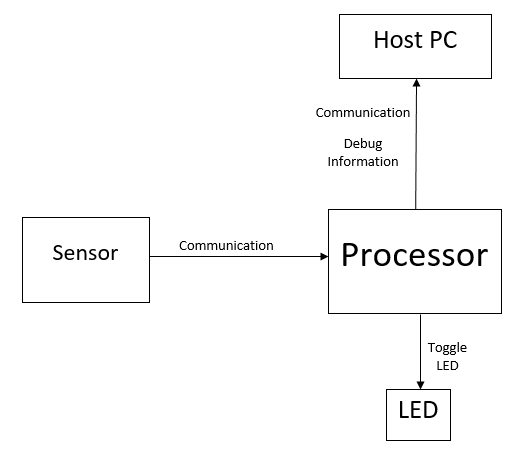
\includegraphics{hardware-schematics-development.pdf}
	\caption{Hardware Block Diagram - Development}
	\label{fig:hardware_schematic_development}
\end{figure}

\begin{figure}
	\centering
	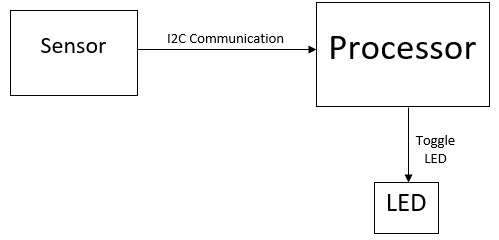
\includegraphics{hardware-schematics-final.pdf}
	\caption{Hardware Block Diagram - Final}
	\label{fig:hardware_schematic_final}
\end{figure}
